\documentclass{article}
\renewcommand\labelenumi{(\theenumi)}
% if you need to pass options to natbib, use, e.g.:
% \PassOptionsToPackage{numbers, compress}{natbib}
% before loading nips_2016
%
% to avoid loading the natbib package, add option nonatbib:
% \usepackage[nonatbib]{nips_2016}

%\usepackage{nips_2016}

% to compile a camera-ready version, add the [final] option, e.g.:
\usepackage[final]{nips_2016}

\usepackage[utf8]{inputenc} % allow utf-8 input
\usepackage[T1]{fontenc}    % use 8-bit T1 fonts
\usepackage{hyperref}       % hyperlinks
\usepackage{url}            % simple URL typesetting
\usepackage{booktabs}       % professional-quality tables
\usepackage{amsfonts}       % blackboard math symbols
\usepackage{nicefrac}       % compact symbols for 1/2, etc.
\usepackage{microtype}      % microtypography
\usepackage{amsmath}
\usepackage{graphicx}

\title{Discovering visual phenomena at multiple scales using the hierarchical Latent Dirichlet Allocation}

\author{
  Genevieve Flaspohler \\
  6.882 - Bayesian Modeling and Inference\\
  \texttt{geflaspo@mit.edu} \\
}

\begin{document}

\maketitle

\begin{abstract}
Marine robots operate in the most communication constrained environment on earth. These challenging conditions require marine robots to display high levels of autonomy. Semantic understanding is an essential precursor to meaningful autonomy. Throughout the scientific community, hierarchical trees appear as a powerful and concise manner of representing complex semantic knowledge. In this work, I apply the nonparametric hierarchical Latent Dirichlet Allocation (hLDA) model to learn a flexible hierarchy over image data collected by the Jaguar AUV during a mission off the Hannibal Sea Mount, Panama to discover hierarchical semantic associations among the observed visual data. 
\end{abstract}

\section{Introduction}
  The Hierarchical Latent Dirichlet Allocation (hLDA) is a topic model introduced by \cite{Blei2010}. Compared to a flat LDA topic model, hLDA is able to model a richer class of hierarchical relationships among topics, while maintaining the nonparametric properties of the popular Hierarchical Dirichlet Process (HDP) topic models.  

The foundation of the hLDA model is the nested Chinese Restaurant Process (nCRP). The nCRP is nonparametric prior over this infinitely deep, infinitely branching tree of topics. Each node $k$ in this infinite tree represents a topic $\beta_k$, and each document in the corpus is defined by a path down the tree $\mathbf{c}_d$. Each path starts with the most general topic at the tree root. Therefore, each document shares this most general topic. The topics in the leaf nodes will be shared by a much more restricted subsets of documents and therefore represent more specific semantic constructs. 

Unlike traditional hierarchical clustering models, parent nodes in the hLDA tree are not summaries of their children. Instead, parent nodes reflect shared terminology amoung their child nodes. For example, every document about sports may contain words such as "score", "team", "win", etc. However, documents about swimming will contain those words \textbf{and} words such as "laps", "pool", "stroke". Documents about tennis will contain the general sports words \textbf{and} words such as "net", "backhand", "serve".  Both the swimming and tennis documents will pass through the general sports node and then through one of the child nodes of the sports nodes, accruing general sports terminology and specific sports terminology respectively. 


\section{The hierarchical LDA Model}
The hLDA model is best described by its generative model, which is reproduced in the Appendix. The generative model draws on several traditional nonparametric constructions: the Chinese Restaurant process (CRP), the stick breaking construction, and the GEM distribution.

\subsection{The nested Chinese Restaurant Process}
The first step in the generative model for documents is to draw a path through the infinitely deep, infinitely branching tree of topics defined by the nCRP prior. This construction is depicted graphically in Figure \ref{fig:ncrp}. The process can be described by the following culinary story. 

A customer enters a city with infinitely many Chinese restaurants. On the first night, she enters the root Chinese restaurant and sits at a table with probability defined by the tradiational Chinese restaurant process parameteried by $\gamma$ (i.e. she sits at an already occupied table with probability proporational to the number of people already sitting at that table and a new table with probaiblity proporational to $\gamma$). At each table in this root restaurant there is a card with the name of another Chinese restaurant in the city. On the second night, our customer goes to the restaurant indicated on that card, and again selects a table according to the traditional CRP, which in turn will have a card with the name of another Chinese restaurant. This process repeats infinitely. Each restaurant in the city is referred to exactly once by a card at another restaurant; thus, the restaurants in the city are organized into an infinitely deep, infinitely branching tree.
 
\begin{figure}[h]
\centering
\includegraphics[scale=0.70]{ncrp}
\caption{CAPTION ME.}
    \label{fig:ncrp}
\end{figure}

\subsection{Generating documents}
After drawing a document's path through the hLDA tree, $\mathbf{c}_d$, according to the nCRP prior, the words in the document are drawn by first assigning each word to a level of the tree $z_{d,n}$, and then drawing a word from the topic distribution $\beta_k$ at the node specified by the document path $\mathbf{c}_d$ and level $z_{d,n}$ within the path. The level distriubion of words for each document $\theta_d$ is sampled from a $\text{GEM}(m, \pi)$ distribution, since the number of levels in the tree is theoretically unbounded. However, in practice, we specify a desired depth of the tree and sample from a truncated $\text{GEM}$ distribution. The full generative model for hLDA presented in \cite{Blei2010} is reproduced in the Appendix.

\subsection{Approximate inference via Gibbs sampling}
Once we have specified a generative model, we can reverse it to recover the optimal parameters settings given observed data. As with many complicated grpahical model, the exact posterior over paratmers given data is not tractable. \cite{Blei2010} introduces a collapsed Gibbs sampler to do approximate inference in the hLDA model. The topic parameters $\beta_k$ and the per-document topic proportions $\theta_d$, are integrated out to speed up the chain's convergence. For each iteration of the sampler, the per-document paths $\mathbf{c}_d$ and the per-word level allocations to topics in those paths $z_{d,n}$ are sampled from the equations reproduced in the Appendix.  Metropolis-Hastings updates are interspersed within Gibbs updates to estimate the relevant model hyperparameters (see Appendix).

\section{Application to marine image data}
Topic modeling algorithms require discrete data, drawn from some vocabulary $\cal V$. These data must be organized into  `documents', collections of discrete data which are assumed to share similar thematic content. The structure imposed by the organization of a corpus into documents is exploited by topic modeling algorithms. From this description, image data appear to be great candidacies for topic modeling. A corpus of images is naturally segmented into topics: an image is a collection of discrete data assumed to share similar thematic content. However, the most naive districtization into pixels, with a vocabulary $\cal V = \{\text{0}, \text{1}, \dots \text{255} \}$ often does not lead to elucidating topic models. This is analogous to modeling text documents with a bag of letters, as opposed to a bag of words.

Instead of using pixels, images are generally modeled using disrectizations at a higher level of abstraction. There are many discrete features that can be extracted from an image, such as SIFT/SURF, ORB, Texton (\cite{Bay:ECCV:2006, RubleeE2011}). In this work, use SURF features to discretized images. SURF features are 128-dimensional floating point features, designed to be invariant to small image perturbations, such as lighting changes or rotation.  Additionally, SURF features contain information about the inherent scale of the feature that can be used for hLDA inference initialization, which will be discussed in Section \ref{sec:init}. An example image from the undersea dataset is shown in Figure \ref{fig:surf} (left), along with the extracted SURF features (right). SURF features are extracted from every image, and $k$-means clustering is applied with $k = 1000$ to produce a discrete vocabulary $\cal V$.

\begin{figure}[h]
\centering
\includegraphics[scale=0.60]{surf}
\caption{CAPTION ME.}
    \label{fig:surf}
\end{figure}

\subsection{Code implementation}
\cite{Blei2010} provides a C implementation of the hLDA collapsed Gibbs sampler. The code expected a bag of words (BOW) list of unique words in each document as input. Given our discretized image data, this code can be applied directly to infer the posterior tree structure. Despite being implemented in C, this inference algorithm runs slowly. One iteration of Gibbs sampling on a corpus of 1,000 images, 3,443,563 total words takes 45 seconds to a minute. Unless otherwise specified, inference was run for 500 iterations of Gibbs sampling for each of five cross-validation runs. Given this time constraint, it was also challenging to experiment with hyperparameter initialization. Results are presented both for manual hyperparmeter selection and using Metropolis-Hastings updates.

\subsection{Algorithm Initialization}
\label{sec:init}
MCMC algorithms guarantee that the stationary distribution of the sampler will converge to the true posterior in the limit of infinite time. However, in the more realistic scenario of limited time, initialization greatly impacts the convergence rate of the algorithm.  In hLDA, the latent space is even larger than in traditional LDA, as it contains both the path assignments to documents and the level assignments to words; good initialization is even more critical. [CITE] suggests using a highly engineered heuristic to determine the inherent scale of image features and then uses this scale to initialize the level of each visual word. I apply a similar approach, using the feature scale already computed for the SURF features.

After calculating the scale for each SURF `word' detected in the image corpus, I apply $k$-means clustering on the feature scales, with $k$ equal to the number of levels in the truncated tree. Larger features are initialized to to higher levels of the tree (closer to the root), where smaller features are assigned to lower levels of the tree. This initialization greatly increased the quality of the posterior tree assigned by inference. The empirical effect of initialization is demonstrated in Figure \ref{fig:init}, in the Appendix.

\section{Empirical Results}
\label{sec:exp}


\subsection{Simulated generative model}
\cite{Blei2010} presents the results of using the hLDA inference procedure to recover model parameters on data simulated from the generative model. I reproduce the simulation results as an initial validation of the inference algorithm and my understanding of the generative model. The experimental procedure and results described fully are in the Appendix.

\subsection{Marine image data}
I discretize the image data from a Jaguar marine robot deployment off the Hannibal Sea Mount, Panama into SURF features and initialize the scale of each feature as described in Section \ref{sec:init}. This mission begins by descending through the water column (1). The robot then passes though a school of fish (2), small rocky terrain (3), larger rocky terrain (4), over porous sandy terrain (5), and then ascends back through the water column (6). The results of running hLDA on this dataset are shown in Figure \ref{fig:run12}. The first row shows example images from that datset. The second row plots human-annotated terrains (water column, biological phenomena, small rocks, large rocks, sandy terrain, etc.). The third row plots the proportion of each topic at a particular time step on the y-axis, calculated as the proportion of words assigned to each topic by the mode tree in an image. Different topics are represented by different colors.  Colors are assigned arbitrarily and have no correspondence between plots. The final row plots the topic proportions discovered by \cite{Girdhar}'s spatiotemporal HDP model, which encodes the spatiotemporal topic consistency assumptions in a video stream and uses ORB features instead of SURF features.

\begin{figure}[h]
\centering
\includegraphics[scale=0.70]{hlda}
\caption{CAPTION ME.}
    \label{fig:run12}
\end{figure}

\section{Discussion}
The hLDA model does not obviously discover a more useful topic distribution when visualized as in Figure 1. For example, the normalized mutual information between the most prevalent topic at each timestep and the human-annotated terrain labels is $0.225$ for the hLDA model and $0.587$ for the spatiotemporal HDP model (SHDP). However, the hLDA model does not have the benefit of any temporal or spatial consistency constraints. This alone could account for the difference between the performance of the SHDP model and hLDA.

The two models also employ different image discretizations: hLDA uses SURF features whereas SHDP uses ORB features. ORB features were uses in SHDP mainly for runtime considerations, since SHDP is also a realtime inference model. Using the more descriptive SURF features should only improve the algorithm's performance. 

Comparing the maximum likelihood topic at each image to a single, ground truth terrain is a very course way of estimating the performance of the topic models on the task we care about: inferring biologically or semantically meaningful structure in a marine robot image stream. This analysis does not fully capture the power of either topic model to classify images as mixtures over global topics. Without more detailed annotation, it is difficult to quantify this aspect exactly. However, empirically, we can observed the topic hierarchy over images discovered by the hLDA model in Figure \ref{fig:tree}. The full tree consists of 68 discovered topics, :w


\begin{figure}[h]
\centering
\includegraphics[scale=0.70]{tree}
\caption{CAPTION ME.}
    \label{fig:tree}
\end{figure}

\newpage

\bibliographystyle{unsrtnat}
\bibliography{hlda,girdhar} \newpage
\section{Appendix}

\subsection{Generative model}
The Hierarchical Latent Dirichlet Allocation (hLDA) model defines the following generative process for documents
%\begin{enumerate}{(1)}
\begin{enumerate}
  \item For each table $ k \in \cal{T}$ in the infinite tree,
  \begin{enumerate}
    \item Draw a topic $\beta_k \sim \text{Dirichlet}(\eta)$
  \end{enumerate}
  \item For each document, $d \in \{1, 2, \dots , D\}$
    \begin{enumerate}
      \item Draw a path through the tree, $\mathbf{c}_d \sim \text{nCRP}(\gamma)$.
      \item Draw a distribution over levels in the tree, $\theta_d | \{m, \pi\} \sim \text{GEM}(m, \pi)$
      \item For each word,
        \begin{enumerate}
          \item Choose level $Z_{d,n} | \theta_d \sim \text{Discrete}(\theta_d)$
          \item Choose word $W_{d,n} | \{ z_{d,n}, \mathbf{c}_d, \beta \} \sim \text{Discrete}(\beta_{\mathbf{c}_d}[z_{d,n}])$, which is parameterized by the topic in position $z_{d,n}$ on the path $\mathbf{c}_d$.
        \end{enumerate}
    \end{enumerate}
\end{enumerate}

\subsection{Gibbs Sampling Updates}
The Gibbs sampler described in \cite{Blei2010} iteratively samples the per-document path assignment variables and the per-word level assignment variables. 
\begin{enumerate}
  \item For each document $d \in \{ 1, \dots , D\}$
  \begin{enumerate}
    \item Randomly draw $\mathbf{c}_d^{(t+1)}$ from Eq. \ref{eq1}
    \item Randomly draw $z_{n,d}^{(t+1)}$ from Eq. \ref{eq2} for each word, $n \in \{1, \dots , N_d\}$
  \end{enumerate}
\end{enumerate}

\subsubsection{Sampling level allocations}
The posterior level assignment for word $n$ in document $d$ can be written as:
\begin{equation}
\begin{split}
  P(z_{d,n} | \mathbf{z}_{-(d,n)}, \mathbf{c}, \mathbf{w}, m, \pi, \eta) & \propto P(z_{d,n} | \mathbf{z}_{d, -n}, m, \pi) P(w_{d,n} | \mathbf{z}, \mathbf{c}, \mathbf{w}_{-(d,n)}, \eta) \\
P(z_{d,n} | \mathbf{z}_{d, -n}, m, \pi) & = \frac{m\pi + \#[\mathbf{z}_{d, -n} = k]}{\pi + \#[\mathbf{z}_{d, -n} \geq k]} \prod_{j = 1}^{k-1} \frac{(1-m)\pi + \#[\mathbf{z}_{d, -n} > j]}{\pi + \#[\mathbf{z}_{d, -n} \geq j]} \\
  P(w_{d,n} | \mathbf{z}, \mathbf{c}, \mathbf{w}_{-(d,n)}, \eta) & \propto \#[\mathbf{z}_{-(d,n)} = z_{d,n}, \mathbf{c}_{z_{d,n}} = c_{d,z_{d,n}}, \mathbf{w}_{-(d,n)} = w_{d,n}] + 
  \eta\\
\end{split}
\label{eq2}
\end{equation}

\subsubsection{Sampling paths}
The posterior level assignment for word $n$ in document $d$ can be written as:
\begin{equation}
\begin{split}
  P(\mathbf{c}_d | \mathbf{w}, \mathbf{c}_{-d}, \mathbf{z}, \eta, \gamma) & \propto P(\mathbf{c}_{d} | \mathbf{c}_{-d}, \gamma) P(\mathbf{w}_{d} | \mathbf{c}, \mathbf{w}_{-d}, \mathbf{z},\eta) \\
  P(\mathbf{c}_{d} | \mathbf{c}_{-d}, \gamma)  & \text{is given by the nCRP prior} \\
  P(\mathbf{w}_{d} | \mathbf{c}, \mathbf{w}_{-d}, \mathbf{z},\eta) & \propto \frac{\prod_w \Gamma (\#[\mathbf{z} = l, \mathbf{c}_{l} = c_{d,l}, \mathbf{w} = w] + \eta}{\Gamma (\sum_w \#[\mathbf{z} = l, \mathbf{c}_{l} = c_{d,l}, \mathbf{w} = w] + V\eta)}\\
\end{split}
\label{eq1}
\end{equation}

\subsection{Simulation Results}
\cite{Blei2010} presents the results of using the hLDA inference procedure to recover model parameters on data simulated from the generative model. In the paper, Blei uses hyperparameter settings $\eta = 0.005$ and $\gamma = 1$ to generate 100 documents of 250 words each. In the simulations, the stick breaking procedure, which determines the depth of the tree, was truncated after three levels; arbitrary branching factor was allowed. 

I implemented the generative model for hLDA \footnote{https://github.com/geflaspohler/hlda/tree/master/generative} and ran it with the same hyperparameter settings. For each tree, Gibbs sampling was run for 10 cross-validation rounds of 5,000 rounds of sampling each. The tree that produced the highest log-likelihood (the "mode") among all the samples in the 10 trials was chosen as the true tree, as described in the paper. However, unlike the results presented in the paper, the provided hLDA code does not seem to recover the true tree structure faithfully. Although the course structure of the tree is well approximated, the details of the lower branches are not recovered. An example of the true simulated tree structure and the structure discovered using inference is shown in Figure \ref{fig:sim}. 

\begin{figure}[h]
\centering
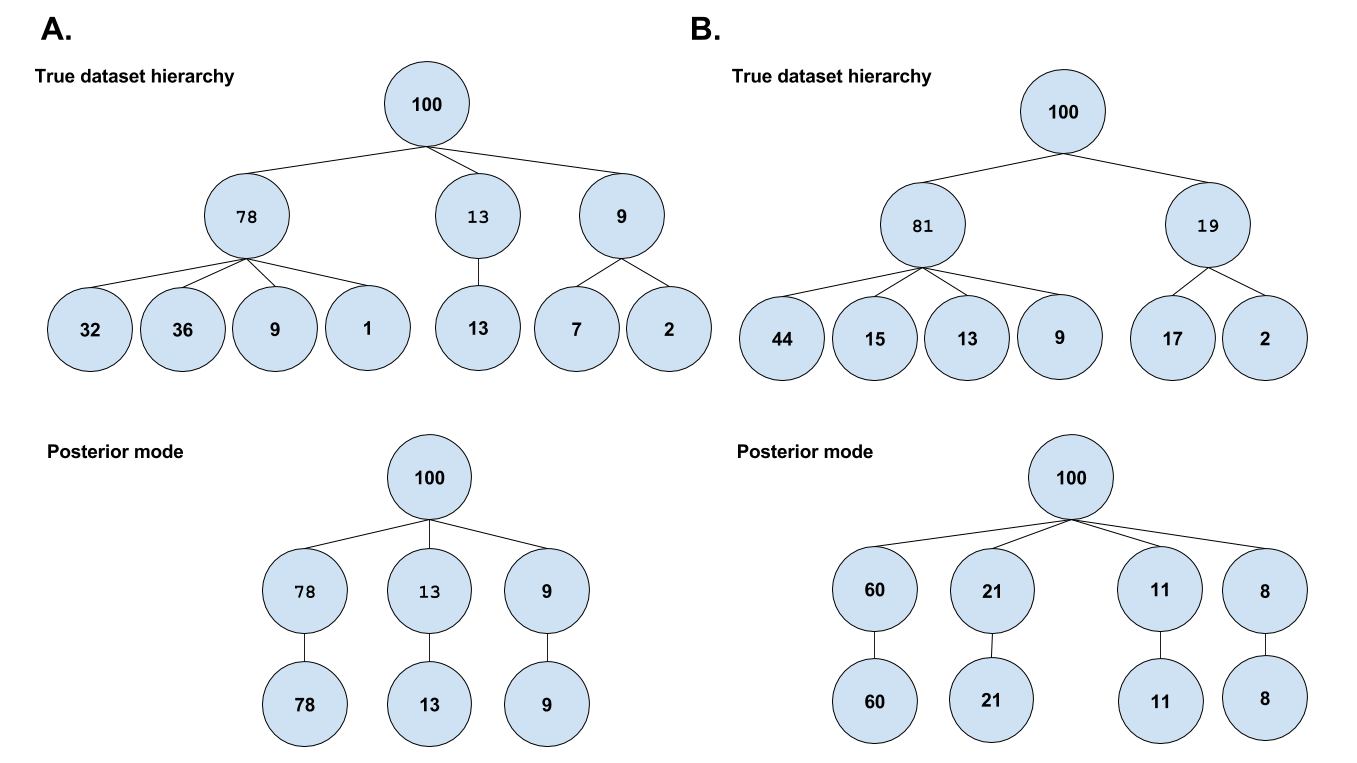
\includegraphics[scale=0.28]{sim_final}
\caption{The results of running hLDA posterior inference on 100 simulated documents and 500 Associated Press news articles. A) The performance of the algorithm on 100 simulated documents, 250 words each. Each node in the tree represents a topic, and the number of documents containing that topic is shown directly on the node. The true topic hierarchy (top) was always smaller than the trees recovered by posterior inference (bottom). B) The three-level topic hierarchy recovered from 500 Associated Press news articles.}
\label{fig:sim}
\end{figure}

\end{document}
